
\chapter{Some distributions}

Statistics is all about comparing our data to the expected distribution of some variable. Whether we are modeling a function of a variable to a specific distribution or assuming a specific sampling distribution, it is always a good idea to have a good working knowledge of distributions.

\section{Discrete distributions}
\label{sec:disdist}

A discrete random variable can only take on positive integer values. Such variables are dichotomous variables such as whether a respondent voted (0 or 1) or a count variable such as the number of children (0, 1, 2, ... etc.). We will revisit these distributions when it comes time to model variables that follow the distribution in Chapter~\ref{sec:logit}.

There are two important concepts for any probability distribution:
\begin{itemize}
\item{The probability mass function}
\item{The cumulative distribution function}
\end{itemize}

The probability mass function (PMF) specifies a probability for observing any one possible value of a random variable, $X$. For example, we can speak of the probability that $X$ is equal to a specific value $x_i$
\begin{equation}
P\left(X=x_i\right)
\end{equation}
and that the sum of the probabilities of all possible values is 1
\begin{equation}
\sum_{i=0}^{\infty} P\left(X=x_i\right) = 1
\end{equation}
We also can talk about the cumulative distribution function, which adds the probabilities for each value of $X$ up to and including a specific value, $x_i$
\begin{equation}
F(x_i)=P\left(X\le x_i\right)
\end{equation}
\subsection{Bernoulli distribution}
\label{sec:bernoilli}
A Bernoulli variable takes on two values, 0 or 1. We are generally interested in the probability of a 1 $(p)$ or the probability of a 0 $(1-p)$. The probability mass function of this distribution is
\begin{equation}
P(x) = p^x\left(1-p\right)^{1-x}
\end{equation}
\subsection{Binomial distribution}
\label{sec:binomial}
We then extend the Bernoulli distribution to consider $n$ Bernoulli events. That is, out of $n$ times, how many instances are 0 or 1? The probability mass function of $k$ events of 1 is
\begin{equation}\label{eq:binomial}
P(k) = {n \choose k}p^k(1-p)^{n-k}
\end{equation}

Figure ~\ref{fig:binomial} illustrates likely distributions of a binomial variable given values for $n$ and $p$.

\begin{figure}
   \centering
   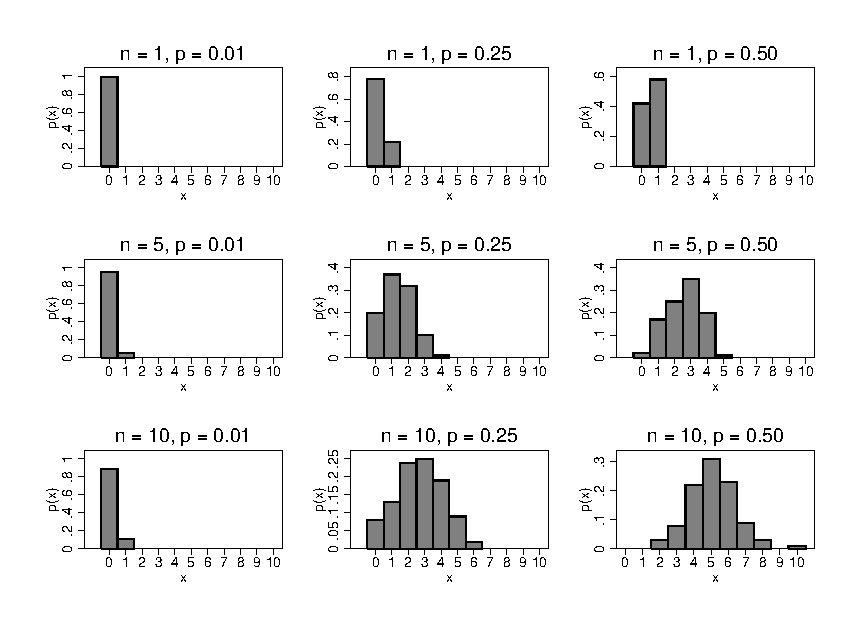
\includegraphics[angle=0,
           width=.75\textwidth]{binomial.eps}
   \caption{Distributions of random binomial variables with different values of $n$ and $p$.}
  \label{fig:binomial}
\end{figure}

\subsection{The Poisson distribution}
\label{sec:poisson}
The Poisson distribution is an extension of the binomial distribution. If we conceive of a parameter $\lambda = np$, where $n$ approaches infinity and $p$ approaches 0 (that is, the first couple trials have a high probability, but as trials increase the probability decreases), then this frequency distribution function becomes
\begin{equation}\label{eq:poisson}
P\left(X=k\right) = \frac{\lambda^k}{k!}e^{-\lambda}
\end{equation}
This distribution if often used to model count data.
\begin{figure}
   \centering
   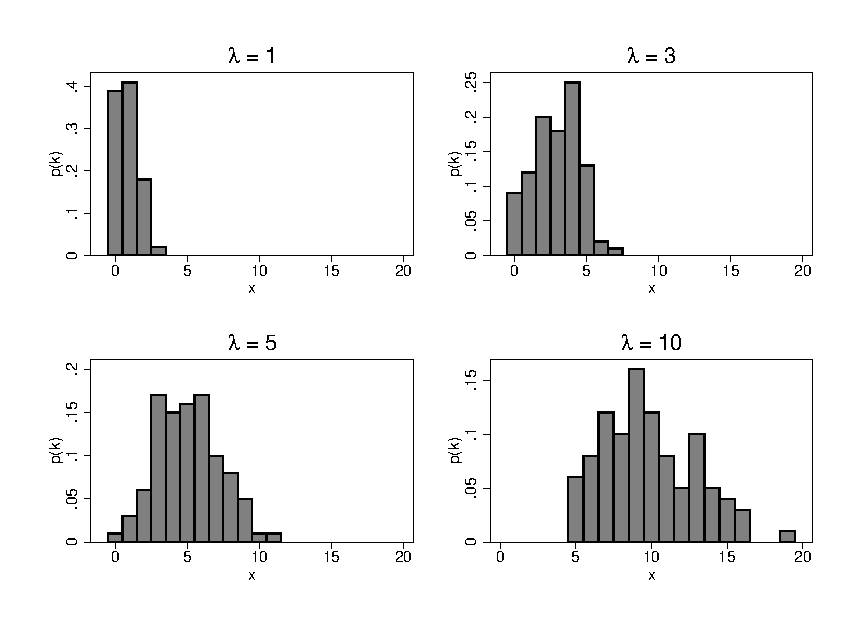
\includegraphics[angle=0,
           width=.75\textwidth]{poisson.eps}
   \caption{Distributions of random Poisson variables with different values of $\lambda$.}
  \label{fig:poisson}
\end{figure}

\subsection{Negative binomial distribution}
\label{sec:negbinomial}
We can extend the Bernoulli distribution to consider a series of Bernoulli events, each with a probability $p$, but ending after $r$ successes (or 1s). That is, out of $n$ times, how many instances are 0 or 1? The probability mass function of $k$ events to get $r$ successes is
\begin{equation}
\label{eq:negbinomial}
P(X=k) = {k-1 \choose r-1}p^r(1-p)^{k-r}
\end{equation}

\section{Continuous distributions}
\label{sec:condist}
The analogous idea to the probability mass function for discrete variables is the probability density function (PDF) that describes continuous variables. These functions have the property that the cumulation of all possible values equals 1. More importantly, we can find the probability that a variable has a value with the interval between $a$ and $b$ by integrating the function
\begin{equation}
P\left(a < X < b\right) = \int_a^b f(x)dx
\end{equation}
Of course, the chance of a specific value is 0
\begin{equation}
P\left(X = c\right) = \int_c^c f(x)dx = 0
\end{equation}
\subsection{The uniform distribution}

A useful distribution is the uniform distribution that spreads the chance of a variable falling between $a$ and $b$ evenly
\begin{equation}
f(x) = \frac{1}{b-a}
\end{equation}

\subsection{The normal distribution}
\label{sec:normaldist}
The big one is the normal distribution. We use this distribution (and others based on it) all statistical tests in regression. We define it with two parameters, $\mu$ and $\sigma$, or the mean and standard deviation.
\begin{equation}
f(x) = \frac{1}{\sigma\sqrt{2\pi}}\mbox{exp}\left[\frac{-\left(x-\mu\right)^2}{2\sigma^2}\right]
\end{equation}
The standard normal is pictured in~\ref{fig:normal}. A standard normal curve is one with $\mu = 0$ and $\sigma = 1$.

\section{Distributions based on the normal distribution}

From here, we move to the major distributions used for statistical tests. The central idea of such distributions is less about describing variables in data, but more describing the sampling distributions of statistics. We encounter these distributions when we consider the probability of observing a statistic (or the data that generated a statistic) assuming a specific null hypothesis in Chapter~\ref{sec:inference}. Note that some details, such as moment generating functions and the gamma distribution are left out, for more details, check out the mathematical statistics text in the bibliography.

\begin{figure}
   \centering
   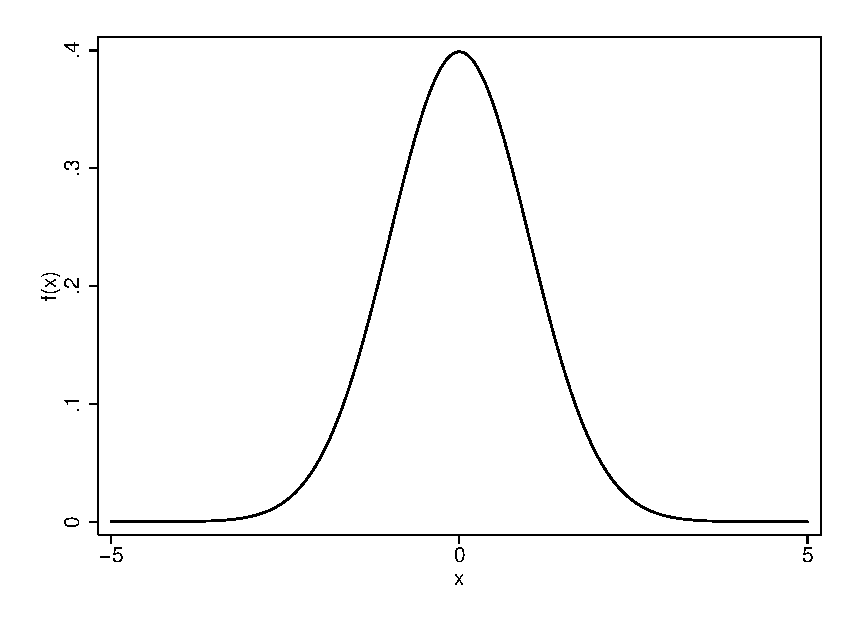
\includegraphics[angle=0,
           width=.75\textwidth]{normal.eps}
   \caption{A variable $x$ distributed $N \sim \left(0,1\right)$.}
  \label{fig:normal}
\end{figure}

\subsection{The $\chi^2$ distribution}

The $\chi^2$ distribution (written chi-square and rhymes with sky-square). This distribution (with 1 degree of freedom) is essentially the square of the normal distributions. That is, if $Z$ is standard normal, then $U = Z^2$ and $U$ is the $\chi^2$ distribution with 1 degree of freedom.

We note the distribution as $\chi_{df}^2$. We can take any normally distributed variable with mean $\mu$ and standard deviation $\sigma$ and transform it into a $chi_1^2$ by transforming it into standard normal and squaring it. That is, if
\[
X \sim N\left(\mu,\sigma\right)
\]
then
\[
\frac{X-\mu}{\sigma} \sim N\left(0,1\right)
\]
so
\[
\left(\frac{X-\mu}{\sigma}\right)^2 \sim \chi_1^2
\]
Formally, the $\chi^2$ distribution employs the gamma function ($\Gamma$) to find the density for any value ($v$) greater than 0 with a certain number of degrees of freedom ($df$):
\begin{equation}
f(v) = \frac{1}{2^{df/2}\Gamma\left(df/2\right)}v^{\left(df/2\right)-1}e^{-v/2}
\end{equation}
Finally, what really makes this distribution useful is that we can {\it add} independent variables' distributions and find the joint probability distribution (again, only if independent). Thus, if $U \sim \chi_n^2$ and $V \sim \chi_m^2$, then $U + V \sim \chi_{n+m}^2$. Thus, you will find many statistics used to evaluate aspects of a regression model will follow a $\chi^2$ distribution.

\begin{figure}
   \centering
   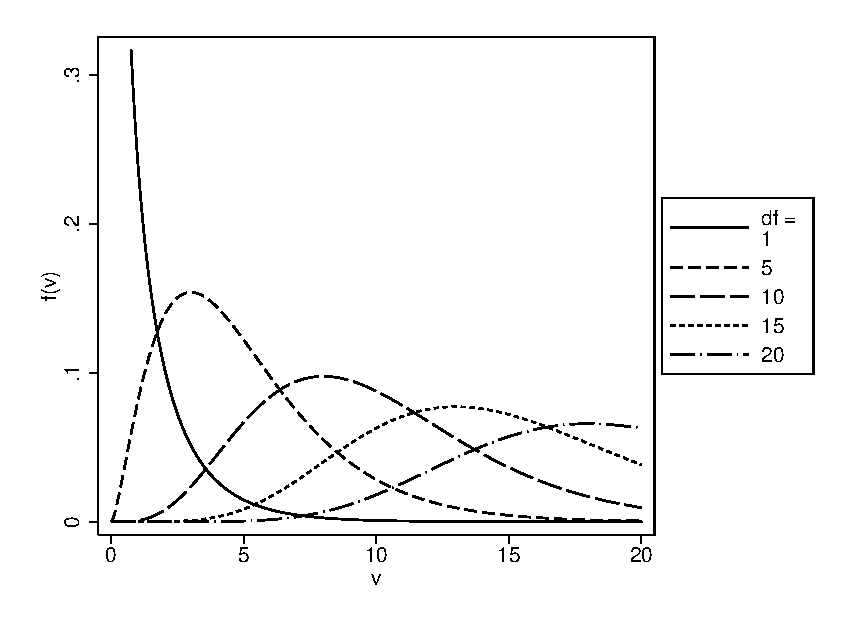
\includegraphics[angle=0,
           width=.75\textwidth]{chi.eps}
   \caption{Plot of $\chi^2$ distribution with various degrees of freedom.}
  \label{fig:chi}
\end{figure}

\subsection{The $t$ distribution}

The distribution you will encounter most often is the $t$ distribution, or sometimes called the "student's" $t$ distribution. This is not because a student derived it, far from it, but it was instead derived by a guy named Gossett in 1908 who was working for Guinness (as in beer) at the time, and published it under the pseudonym "student" for various reasons.

The $t$ distribution essentially works like the normal distribution, except it takes into account the small(er) sample sizes often used in research. If independent variables $Z \sim N\left(0,1\right)$ and $U \sim \chi_{df}^2$, then the $t$ distribution is the ratio of the normal $Z$ to the square root of the ratio of $\chi^2 U$ with $df$ degrees of freedom to $df$, or $t = \frac{Z}{\sqrt{U/df}}$.

Again, using the gamma function, this can we written as the following density function
\begin{equation}
f(t) = \frac{\Gamma\left(\frac{df+1}{2}\right)}{\sqrt{df\pi}\Gamma\left(\frac{df}{2}\right)}\left(1+\frac{t^2}{df}\right)^{\frac{-\left(df+1\right)}{2}}
\end{equation}

\begin{figure}
   \centering
   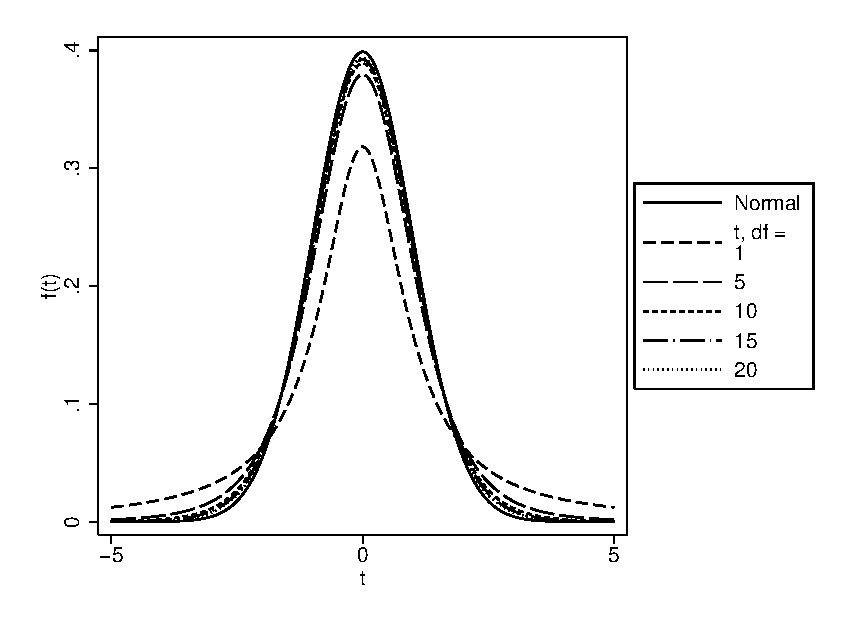
\includegraphics[angle=0,
           width=.75\textwidth]{tdist.eps}
   \caption{Plot of the normal distribution and two $t$ distributions with various degrees of freedom}
  \label{fig:tdist}
\end{figure}

\subsection{The $F$ distribution}

Finally, we have the $F$ distribution. If we have two independent $\chi^2$ variables, $U$ and $V$, distributed with $m$ and $n$ degrees of freedom respectively, then $F=\frac{U/m}{V/n}$, or formally for all positive values of $F$,
\begin{equation}
f(F) = \frac{\Gamma\left(\frac{m+n}{2}\right)}{\Gamma\left(\frac{m}{2}\right)\Gamma\left(\frac{n}{2}\right)}\left(\frac{m}{n}\right)^{\frac{m}{2}}F^{\frac{m}{2}-1}\left(1+\frac{m}{n}F\right)^{\frac{-\left(m+n\right)}{2}}
\end{equation}
\subsection{Who cares?}
There are several notable aspects of statistical analysis that make all these distributions based on the normal curve important. First, means and variances are independent with normally distributed variables, making modeling them in regressions very easy. Second, variances follow $\chi^2$ distributions, making the $F$-distribution appropriate for the ratio of variances.


\begin{figure}
   \centering
   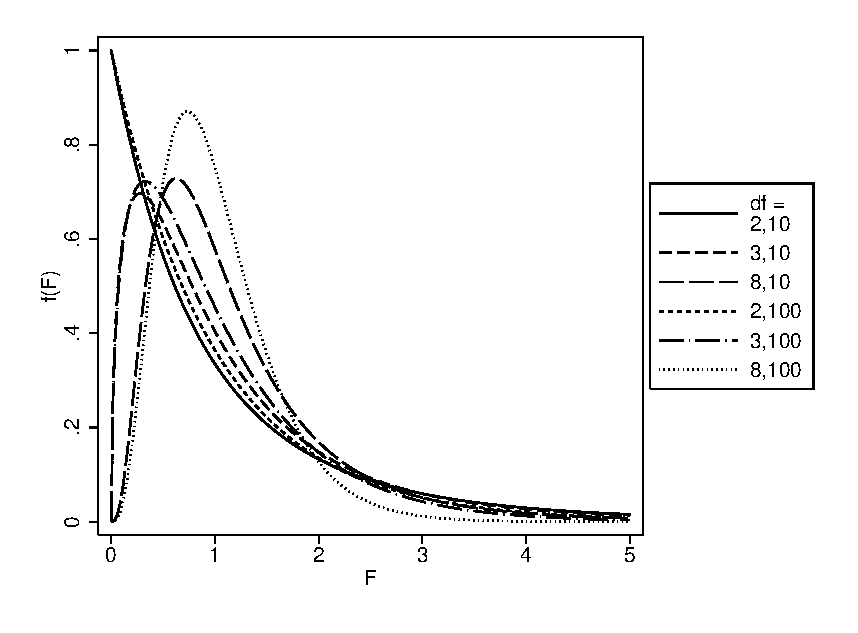
\includegraphics[angle=0,
           width=.75\textwidth]{f.eps}
   \caption{Plots of $F$ distribution with various degrees of freedom combinations.}
  \label{fig:f}
\end{figure}

